\chapter{Software}


\section{HTML5}

\section*{Erläuterung}
HTML5 ist die fünfte Generation der Hypertext Markup Language. HTML wird hauptsächlich zur Darstellung von Websites im Internet genutzt. Die HTML-Dateien werden dabei von einem Browser abgerufen und dargestellt.

\section*{Funktionalität}
Dadurch das HTML mit CSS und JavaScript um ein Design und Funktionen erweitert werden kann ist es sehr flexibel und vielseitig einsetzbar. Ganze Programme werden heute als WebApp programmiert und bieten denselben Funktionsumfang wie normale desktopbasierte Programme. Weil nur ein Browser benötigt wird um die Websites darzustellen sind sie außerdem plattformunabhängig.  


\section*{Verwendung}
HTML bildet das Fundament für den Bad-Designer, auf dem alle anderen Features aufbauen. Die Modelle der sanitären Anlagen werden hier geladen. Die restlichen Funktionen werden mit JavaScript implementiert.

\newpage
\clearpage

\section{JavaScript}

\section*{Erläuterung}
JavaScript ist eine Skriptsprache, die dazu dient, um HTML zu erweitern. Damit kann man auf Benutzerinteraktionen reagieren und auswerten, Inhalte verändern, generieren und nachladen. Somit sind die Seiten dynamisch und ergänzen HTML und CSS so dass sie interaktiv werden. Des Weiteren wird JavaScript auch für Server und Microcontroller verwendet. Eine bekannte serverseitige Plattform, nämlich Node.js, basiert auf der JavaScript-Laufzeitumgebung. 
\\
Die Syntax der 1995 erschienenen Sprache ähnelt der von C. Obwohl Java auf Gemeinsamkeiten vermuten lässt ist JavaScript deutlich anders und vieles abweichend implementiert. Durch die Variabilität ist es möglich objektorientiert, prozedural oder funktional zu programmieren.

\section*{Funktionalität}
JavaScript bildet mit seinen umfangreichen Funktionen ein Grundgerüst für die meisten Dinge. Animationen, Berechnungen, Benutzer Interaktionen und Datenverarbeitung werden es dadurch möglich.


\section*{Verwendung}
Das Laden der Modelle, Animationen, Benutzer Eingaben und Berechnungen wurden allesamt in JavaScript realisiert. JavaScript ist der wichtigste Bestandteil der Arbeit, die meisten Funktionen wären ohne diese Skriptsprache nicht möglich.  Außerdem basiert die Bibliothek three.js auf dieser Sprache und erweitert sie. Mehr zu three.js wird auf den folgenden Seiten näher erläutert.


\newpage
\clearpage


\section{WebGL}

\section*{Erläuterung}
WebGL, kurz für Web Graphics Library, ist eine auf JavaScript basierende Programmierschnittstelle, die es ermöglicht 3D-Grafiken hardwarebeschleunigt im Webbrowser ohne zusätzliche Erweiterungen, Bibliotheken und Technologien darzustellen. Des Weiteren basiert WebGL auf den Spezifikationen von OpenGL ES, kurz für Open Graphics Library for Embedded Systems. Diese beschreibt eine plattform- und sprachenunabhängige Programmierschnittstelle für die Entwicklung von 3D-Computergrafiken. 
\\
Die 2011 erschienene Library ist lizenzfrei von der Khronos Group und Mozilla entwickelt worden. Mit der Zeit haben immer mehr Unternehmen die Entwicklung unterstützt, dazu zählen unteranderem Google Chrome, AMD, Ericsson, Nvidia und Opera. 


\section*{Funktionalität}
Dadurch das die Grafik-Bibliothek im Browser läuft, ist sie plattformunabhängig und hat unteranderem deshalb auch eine große Reichweite. Zusätzlich gestattet sie Grafikern mit den beliebten Softwarewerkzeugen wie Blender, Maya oder CopperCube zu arbeiten ohne sich um die Darstellung anschließend kümmern zu müssen. WebGL konfiguriert und verarbeitet die Modelle für den Browser.

\section*{Verwendung}
WebGL kann für eine Vielzahl von Dingen verwendet werden, durch immer leistungsfähigere Geräte und Anwendungen wird das Anwendungsgebiet größer. Hauptsächlich wird es für 3D Modelle im Internet genutzt. Vor allem im Marketing Bereich wird die Anwendung kontinuierlich beliebter, da die Hersteller nun die Möglichkeit haben dem Kunden das Produkt auf einem zwei dimensionalen Bildschirm drei dimensional darzustellen. Dadurch steigt die Verkaufswahrscheinlichkeit wesentlich an da der Kunde eine Übersicht bekommt als hätte er sich das Produkt in echt angesehen.
\\
Das Laden der Badezimmer-Module übernimmt WebGL und dient gleichzeitig als Basis für three.js. Die ganzen Animationen und Effekte werden von dieser Bibliothek abgewickelt.



\newpage
\clearpage  

\section{NGINX}\label{sec:NGINX}
\section*{Erläuterung} 
NGINX ist eine modular aufgebaute Webserver-Software, die von Igor Sysoev entwickelt wurde. Sie wird unter der BSD-Lizenz[\ref{sec:BSD}] entwickelt. Die Software ist das erste Mal Ende 2004 erschienen und wird bis heute in regelmäßigen Abständen aktualisiert und weiterentwickelt. Außerdem wurde er in der weitverbreiteten und robusten Programmiersprache C geschrieben.

\section*{Funktionalität}
Der Webserver bietet durch den modularen Aufbau eine Vielzahl an möglichen Techniken, wie zum Beispiel Lastverteilung, Reverse proxying, SSL, Flash-Video-Streaming, WebSocket-Protokoll und vieles mehr. 


\section*{Verwendung}
NGINX gehört zu den marktführen und wird heutzutage bei rund
 42\% der 1.000 Webseiten ~\cite{nginxWorldWide} mit dem höchsten Traffic verwendet. 
 Als http-Server hat er in Österreich sogar knapp 10\% Marktanteil ~\cite{nginxAT}. 
\\
Der Webserver dient beim Bad-Designer als Back-End wo die ganzen Modelle vom Bad und die Website selbst gehostet werden.



\newpage
\clearpage

\section{AutoCAD}

\section*{Erläuterung}
AutoCAD ist ein von AutoDesk entwickelter grafischer Zeichungseditor. Dieser ermöglicht es speziell technische Zeichnungen zu modellieren. Außerdem ist es ein vektororientiertes Zeichentool, das auf den Grundlagen für komplizierte 3D-Objekte basiert wie Linien, Polylinien, Kreisen, Bögen und Texten.
\\
Durch die umfangreichen 3D-Funktionen findet das Programm primär in den Bereichen Maschinenbau, Architektur, Design, Geoinformatik häufig Verwendung. In den genannten Bereichen ist die Software konstitutiv und manche Bauwerke beziehungsweise Maschinen sind erst dadurch möglich gewesen.

\section*{Funktionalität}
Die von der Firma AutoDesk entwickelten Dateiformate .dwg sowie .dxf sind mittlerweile ein Industriestandard im Austausch von CAD-Daten. Dies ermöglicht es das die Dateien auf den verschiedensten Plattformen wie Windows, Unix und MacOS mit Hilfe des Editors verwendbar sind. Desweitern kann man es auch als WebApp und Mobile App für Smartphones und Tablets verwenden.

\section*{Verwendung}
Alle Module des Badezimmers sind in AutoCAD modelliert worden. Von den Registern bis hin zu den Modulen des Bades. Die sanitären Anlagen wurden von der Firma {\projectpartner} zur Verfügung gestellt.



\newpage

\begin{figure}
	\begin{center}
		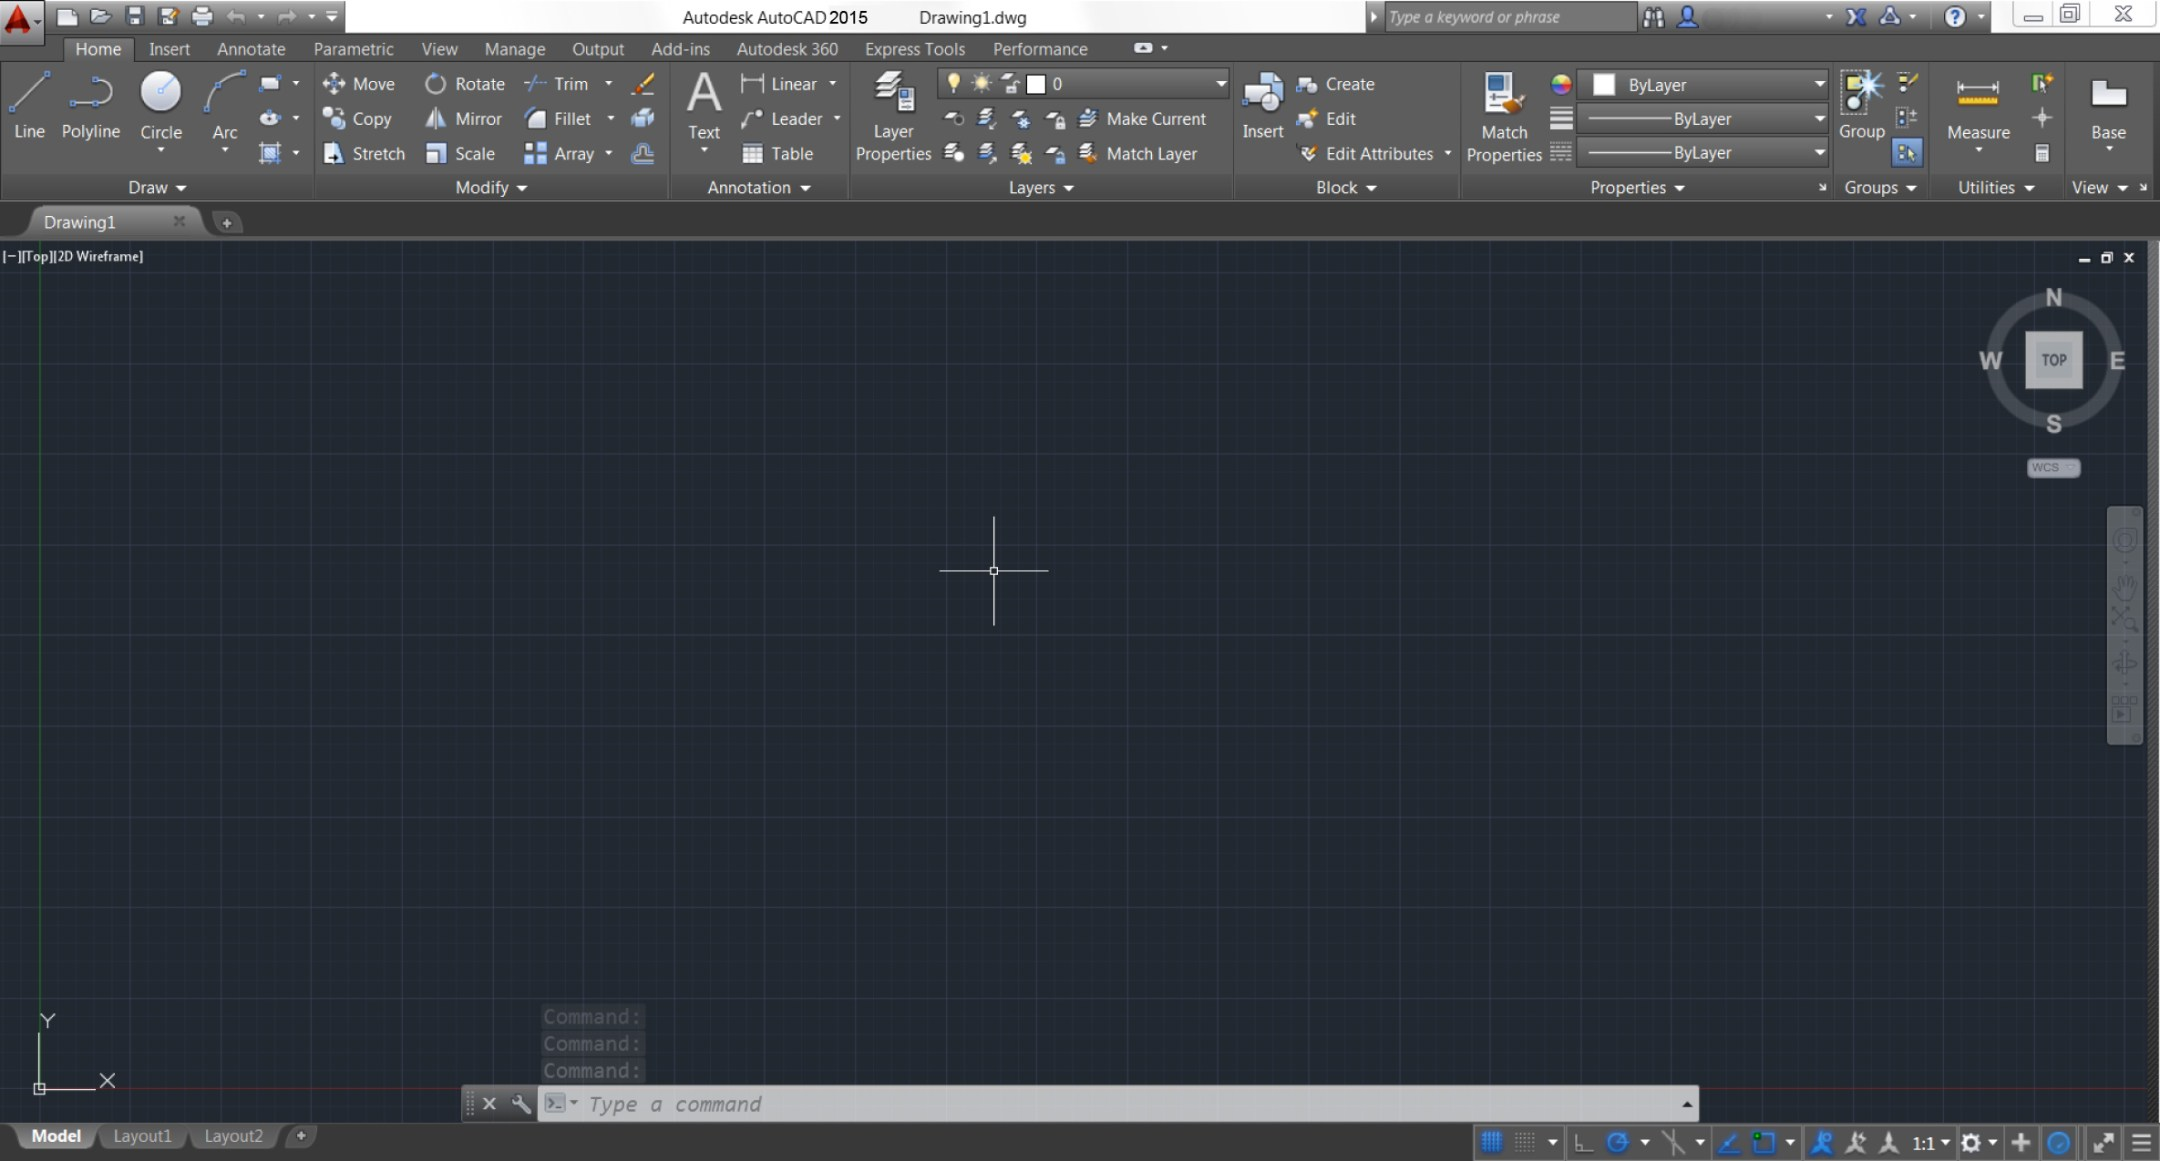
\includegraphics[width=16cm]{images/AutoCAD_UI.jpg}
		\caption{AutoCAD UI ~\cite{autocad}}
	\end{center}
\end{figure}


\newpage
\clearpage

\section{Electron}\label{sec:Electron}



\section*{Erläuterung}
Electron ist ein auf C++ und JavaScript basierendes quelloffenes Framework entwickelt von GitHub. Das 2013 erstmals erschienene Framework wird unter der MIT-Lizenz [\ref{sec:MIT}] vertrieben. Die auf Chromium und Node.js basierende Architektur ermöglicht es eine Cross-Platform-Desktop-Anwendung zu realisieren.

\section*{Funktionalität}
Webseiten die in HTML, CSS und JavaScript geschrieben wurden, können mit Electron in Desktop Anwendung umgewandelt werden ohne erheblichen Aufwand. Des Weiteren ist es möglich mit anderen Frameworks wie Vue.js und Angular zu arbeiten und anschließend zu einer Desktop App konvertieren. Das besondere daran ist, dass alle Electron-Executable auf den Betriebssystemen Windows, MacOS und Linux einwandfrei ohne Zutun ausführbar sind.


\section*{Verwendung}
Viele weitverbreitete und bekannte Programme wie die beliebten Editoren Atom und VS Code als auch die Messenger Discord und Skype wurden in Electron erstellt.
\\
Das Framework erlaubt es den Bad-Designer ohne eine Internetverbindung und lokal auf dem Rechner laufen zu lassen. Dafür muss nur das Executable heruntergeladen werden und schon ist es einsatzbereit.


\begin{figure}
	\begin{center}
		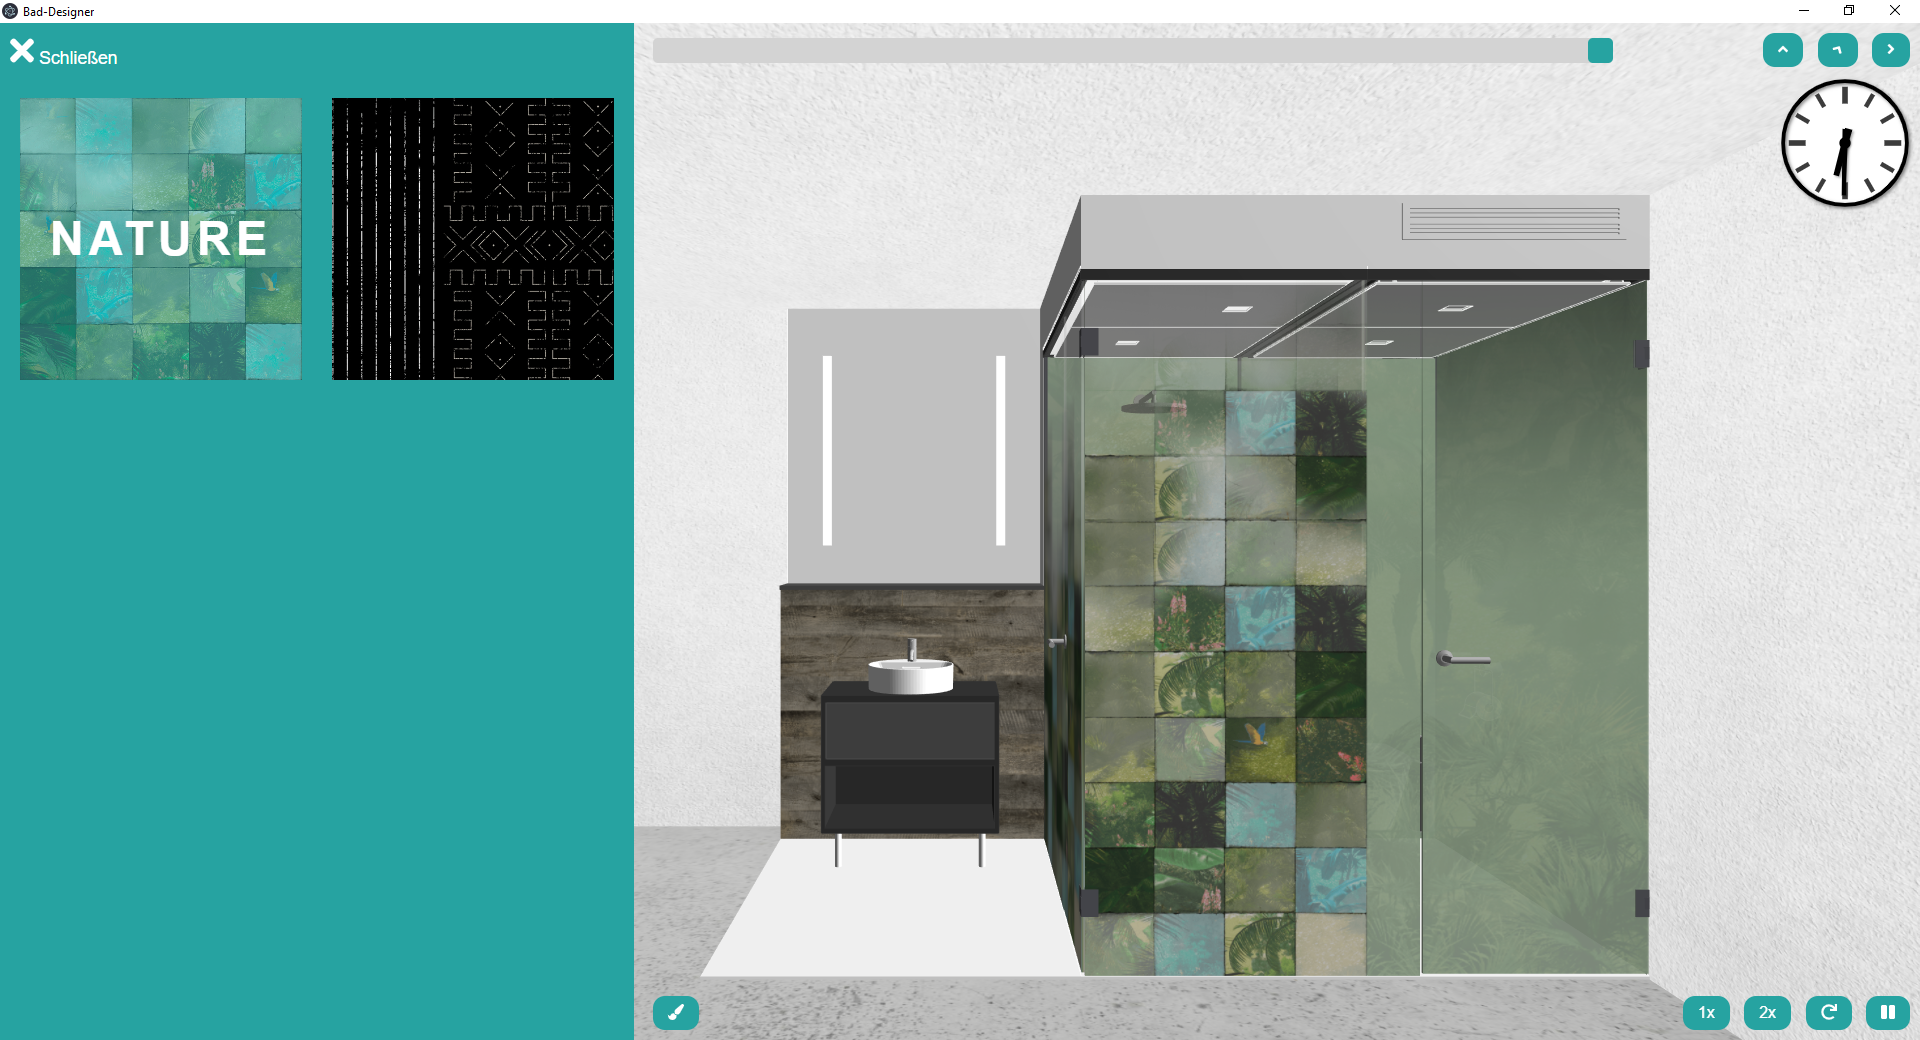
\includegraphics[width=16cm]{images/Electron_BD.png}
		\caption{Bad-Designer als Electron Anwendung}

	\end{center}
\end{figure}


\newpage
\clearpage
\section{Git}
\section*{Historie}
Git ist eine kostenlose Software, die für die verteilte Versionsverteilung von Dateien entwickelt wurde. Git wurde vom Linux-Kernel-Entwickler Linus Torvalds initiiert und entwickelt. Torvalds kam auf diese Idee da er zuvor BitKeeper nutzte, diese aber durch Lizenzänderungen kostenpflichtig wurde. 2005 begann er mit der Entwicklung des beliebten Versionsverwaltungsprogrammes. Dabei hatte er drei Anforderungen. Er wollte Unterstützung verteilter Arbeitsläufe, hohe Sicherheit gegen Verfälschung und hohe Effizienz. Mittlerweile ist der Maintainer Junio Hamano. 2018 wurde GitHub für 7,5 Milliarden US-Dollar von Microsoft übernommen. \\
Git läuft auf den Betriebssystemen Linux, MacOS und Windows. Das Programm selbst wurde in den Sprachen C, Perl, Tcl, Python und C++ geschrieben und unter der GNU-Lizenz [\ref{sec:GNU}] veröffentlicht. 
\\
Zu den Mitbewerbern von Git gehören GitLab und BitBucket. Laut der Plattform Open Hub, eine Website zur Katalogisierung von open-source-software, verwenden dort 71\% aller registrierten Projekte Git. \cite{GitMarketshare}
\\
Der Name stammt aus der britischen Umgangssprache der so viel wie Blödmann bedeutet. Torvalds wählte diesen Namen, weil er in der Softwarewelt unbenutzt war, kurz ist und er mit dem Namen einen Witz über sich selbst machte.
\\
\begin{quote}
	“I’m an egotistical bastard, and I name all my projects after myself. First ‘Linux’, now ‘Git’.” – \textbf{Linus Torvalds} \cite{TorvaldsJoke} 
\end{quote}
\clearpage
\newpage
\section*{Eigenschaften und Besonderheiten}
\subsection*{Branching}
Ein fester Bestandteil und Besonderheit an Git ist das Branching. Ein Branch ist dabei ein neuer Entwicklungszweig, dies ermöglicht es unabhängig vom Hauptzweig zu entwickeln und anschließend beide Zweige oder mehrere zu vereinen, dass sogenannte merging. Diese Verzweigungen sind in Git besonders effektiv implementiert, da sie lediglich eine Referenz auf einen bestimmten Commit sind.



\begin{figure}[!b]
	\begin{center}
		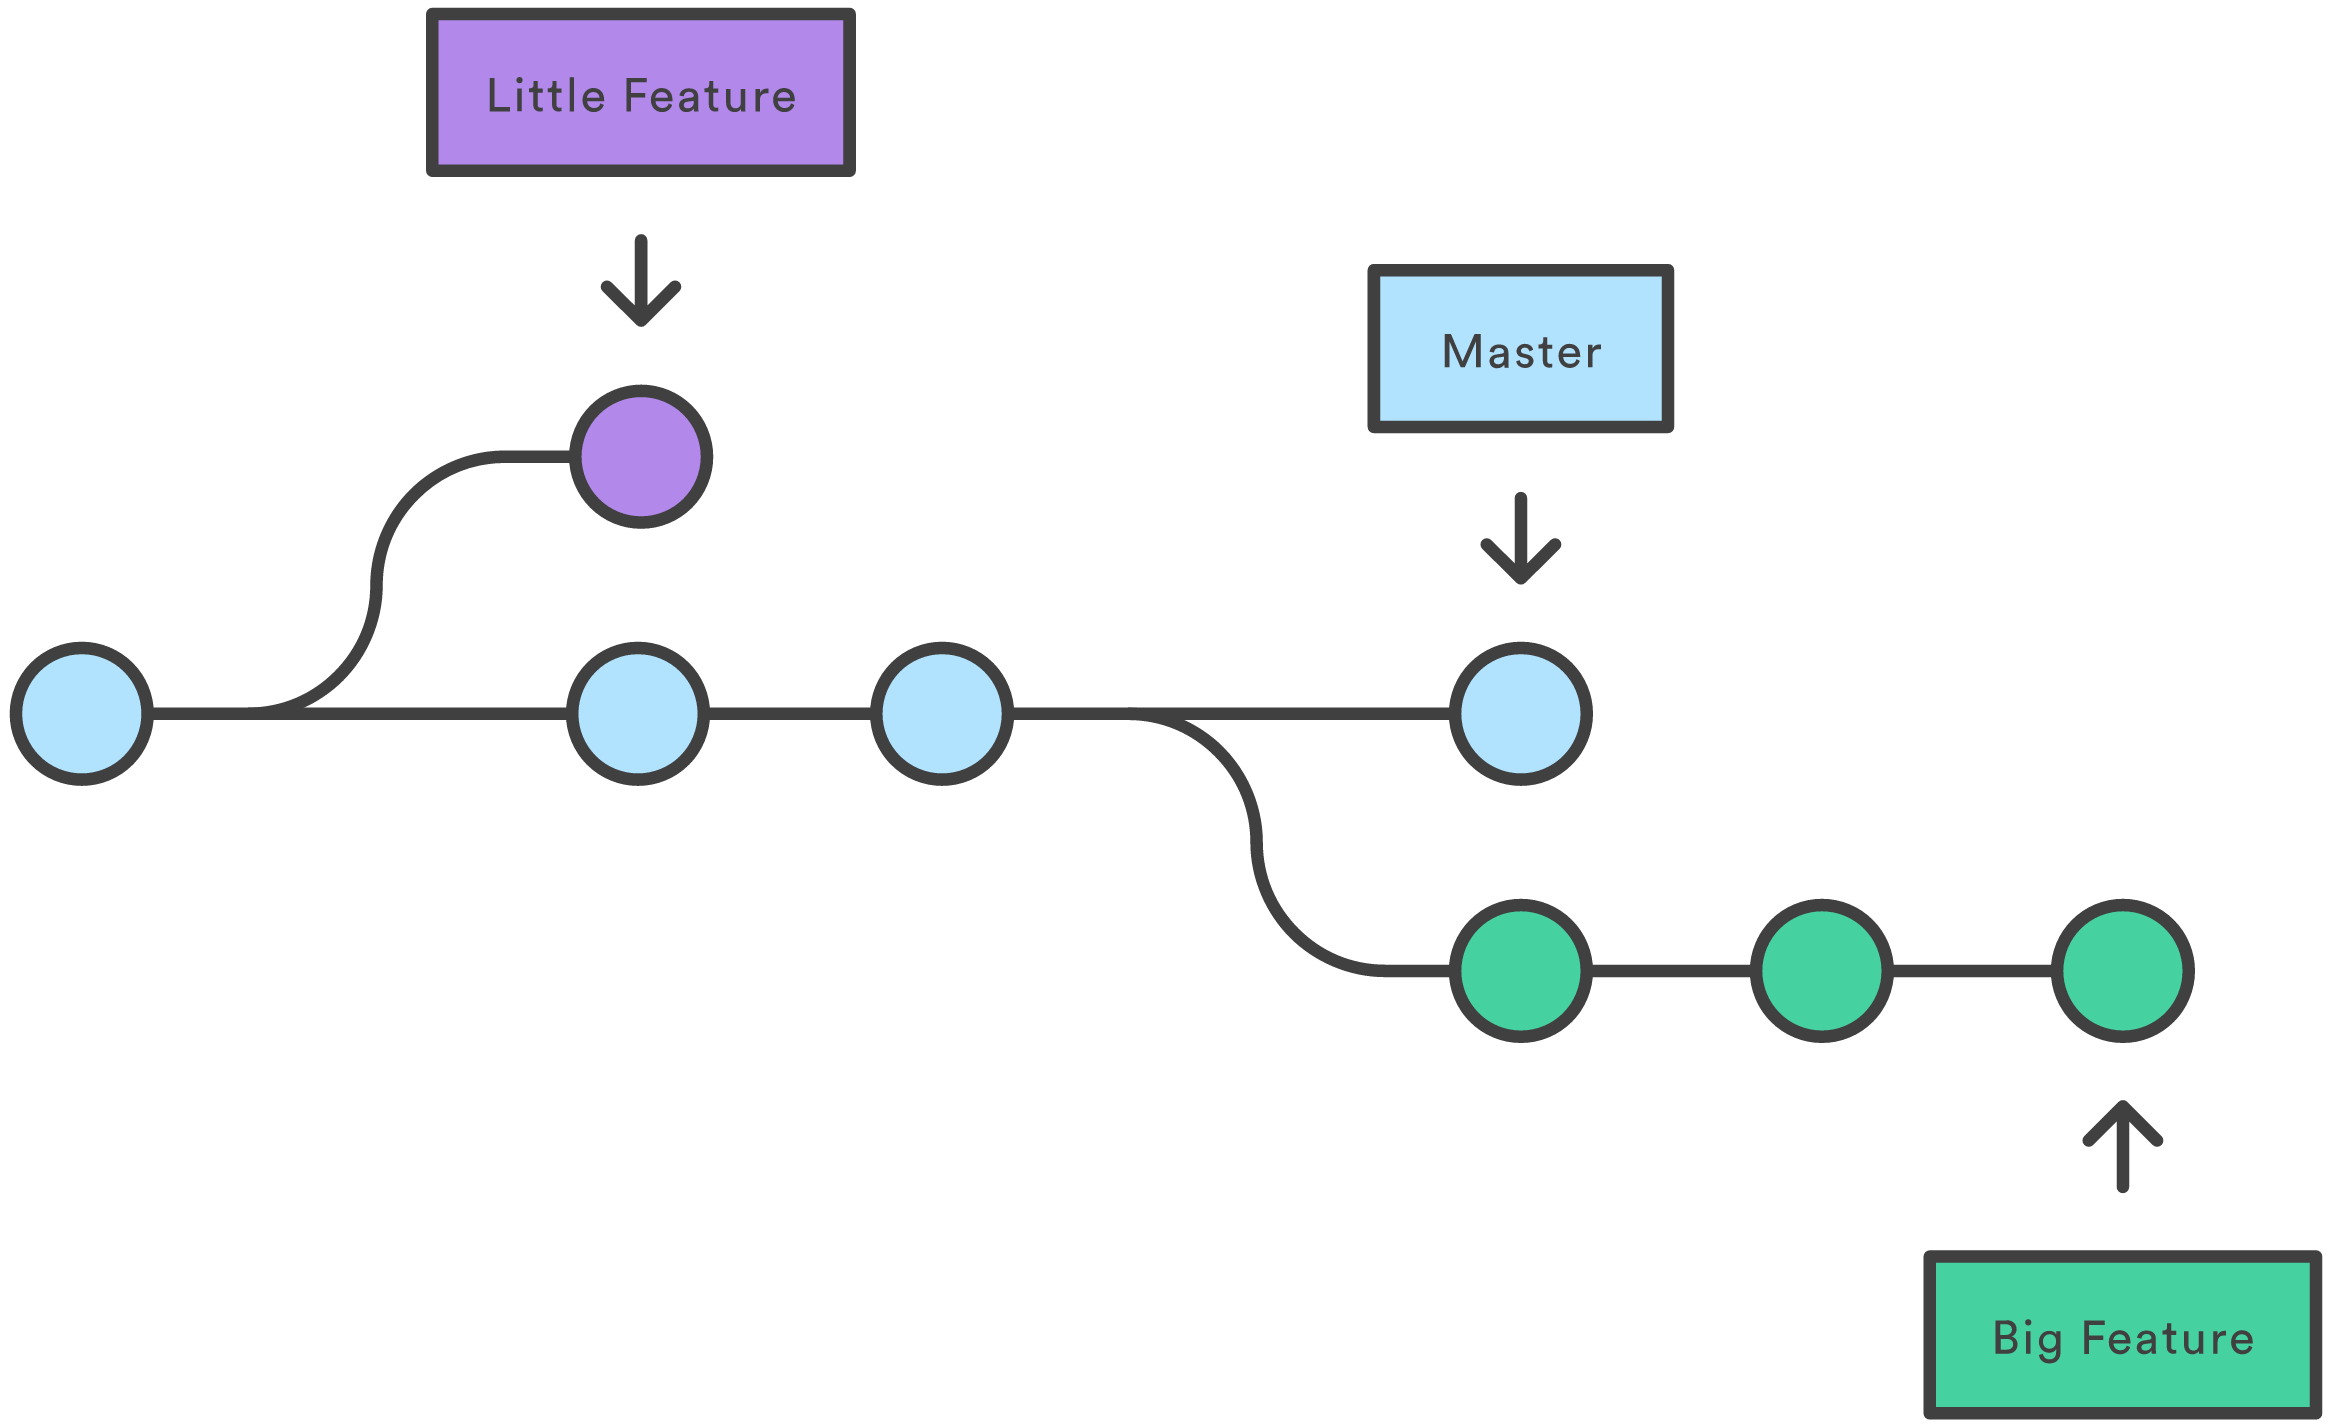
\includegraphics[width=16cm]{images/Git-Branches-1.png}
		\caption{Visualisierung von Zweigen in Git ~\cite{GitBranches}}
	\end{center}
\end{figure}
\newpage
\subsection*{Dezentralisierung}
Dadurch das jeder Benutzer sich eine lokale Kopie des Repositories samt Versionsgeschichte herunterladen kann, können die meisten Operationen ohne Internet durchgeführt werden. 

\subsection*{Sicherer Datentransfer}
Git bietet eine Vielzahl an unterschiedlichen Netzwerkprotokollen, um Daten zwischen Repositories zu übertragen. Das gängigste ist aber das sichere SSH Protokoll für Schreiboperationen und ein eigens entwickeltes Protokoll für das Fetchen und Clonen genutzt wird.

\subsection*{Sicherung der Projektgeschichte}
In Git ist es nicht möglich die Versionsgeschichte zu manipulieren. Das ist dem Hash-Wert geschuldet der bei jeder Revision (Commit) gespeichert wird. Dieser Wert basiert immer auf der vollständigen Geschichte, die bis zu jener Revision vorangegangen ist. 


